\section{Standards, Constraints and  Milestones }

\subsection{Standards (Sustainability)}
In our study, we used machine learning which is one such field that considered where sub problems are analyzed. For example, to make a decision, prediction, clustering, similarity learning, metric learning, reinforcement learning, classification, deep-learning and so many. Using machine learning algorithms such as CNN,Support Vector Machine, Random Forest, Decision tree, Linear Regression, Logistic Regression, KNN, K-Means is easy and efficient to develop a model. Each algorithm has its properties. In this paper, we applied  CNN and classify 80-20 rules and augmented the data. Every algorithm gave us better accuracy. Just choosing an algorithm doesn't make a model efficient and smooth. It also needs a standard dataset. To make standard data, the dataset needs to be prepossessed which means there will be no redundant data, no null data, no inconsistent data, no duplicate data. After that, necessary feature will be extracted. And in the future, if we add new more features, the recognization may be more accurate than it is now. Because inaccessibility of data, some features aren't added. 

\subsection{Impacts on Society }
Handwritten digit recognition is the ability of a computer to recognize the human handwritten digits from different sources like images, papers, touch screens, etc, and classify them into 10 predefined classes (0-9). This has been a topic of boundless-research in the field of deep learning.The applications of digit recognition include in postal mail sorting, bank check processing, form data entry, etc. The main problem lies within the ability on developing an efficient algorithm that can recognize hand written digits, which is submitted by users by the way of a scanner, tablet, and other digital devices.Which is important for our society.

\subsection{Ethics}
Depending on the information implemented to develop the model, this recognition framework encompasses a larger utilization level. The utilization of recognition of digit needs to maintain individuals’ security concerns and ought not to be utilized for any reason that puts a national or social safety vulnerability. All the work like utilization, collection of the dataset needs to complete under the code of moral standards.

\subsection{Challenges}
The issue is that there's a wide range of handwriting – good and bad. This makes it tricky for programmers to provide enough examples of how every character might look. Plus, sometimes, characters look very similar, making it hard for a computer to recognise accurately..



\subsection{Constraints}

\textbf{Design Constraints: } The overall structure of the recommended architecture can be executed based on historical data. The model needs systems with high processing capacity to recognize the handwritten digit.

\textbf{Component Constraints: } The component requirements of the recommended architecture include,
\begin{itemize}
\item Minimum Processor Requirement:  Intel i3
\item Minimum Memory Requirement: 4GB 
\item Anaconda Environment
\item Jupyter Notebook
\end{itemize}


\textbf{Budget Constraints: }The cost of completing our research which is the recognizing the handwriting digit recognize  don't need any additional purchases for hardware and software.

\subsection{Timeline and Gantt Chart}
We divided the timeline into three segments to complete this thesis work based on the three-semester. In the first semester, we reviewed the related work of the thesis topic and then we proposed a model based on our planning. In the second semester, we collected the data and analyzed them, and deciding how to use our proposed model. In the third semester, we implement and test our proposed model and complete the report writing based on all over the timeline.

Figure \ref{fig18} contains the Gantt chart describing the work execution process of the thesis
work. The thesis work’s overall execution is three semesters long, where each semester
is twelve weeks long.

\begin{figure}[htbp]
\centerline{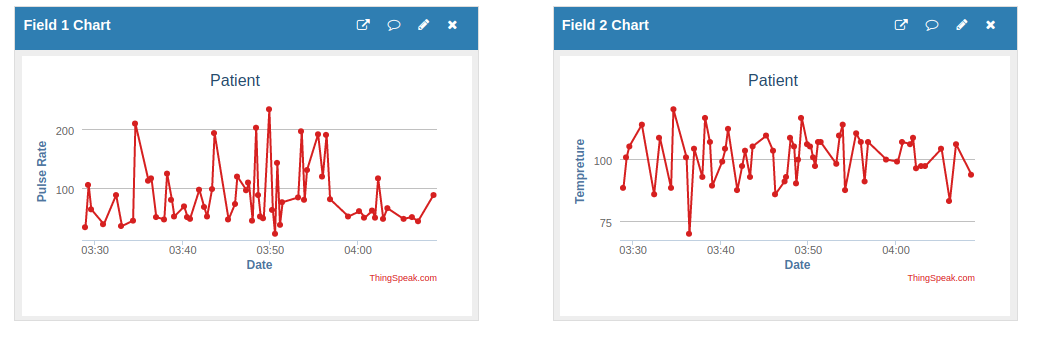
\includegraphics[scale=0.83]{chart.png}}
\caption{Gantt chart of the work execution process }
\label{fig18}
\end{figure}

\vspace{100mm}


\subsection{Summary}
Although it should be noted, despite our lack of data, prediction of player's performance can be a well-suited complement to other methods. We've already explained that a team is selected manually by the team manager. They don't analyze the previous record of player's which is a major cause of losing a game. But it isn't be guaranteed that the selected player can do well in a match. It is happening due to the deficiency of data. The proposed system prediction of player's performance architecture can be implemented in lightweight tools that are free and convenient.